% samplepaper.tex: springer.com
% modificato da MM 06/05/2018
%
\documentclass[runningheads]{llncs}


\usepackage[a4paper, total={6in, 9in}]{geometry}


\usepackage[italian]{babel}
\usepackage{graphicx}
\usepackage{listings}
\usepackage{threeparttable}
\usepackage{tipa}
\usepackage{tikz}
\usepackage{subfig}
\usepackage{graphicx} % for "\includegraphics" macro
% Used for displaying a sample figure. If possible, figure files
% should be included in EPS format.  If you use the hyperref package,
% please uncomment the following line to display URLs in blue roman
% font according to Springer's eBook style:
% \renewcommand\UrlFont{\color{blue}\rmfamily}
\begin{document}
%
\title{Classificazione articoli ANSA via topic modelling}
%
% \titlerunning{Abbreviated paper title}
% If the paper title is too long for the running head, you can set
% an abbreviated paper title here
%
\author{%
  Alessandro Stefani\inst{1} e
  Cristi Gutu\inst{2}}
%
\authorrunning{Alessandro Stefani, Cristi Gutu}
% First names are abbreviated in the running head.  If there are more
% than two authors, 'et al.' is used.
%
\institute{Corso di laurea in Statistica per le tecnologie e le scienze
%\footnote{famoso persuasore sulla piattaforma Tinder, swipe right @asteph7cd}
  matricola 1148387 \email{alessandro.stefani.6@studenti.unipd.it} \and Corso di laurea in Statistica per le tecnologie e le scienze,
      matricola 1147351 \email{gheorghecristi.gutu@studenti.unipd.it}
  }
%
\maketitle
% typeset the header of the contribution
%
\begin{abstract}
In questo progetto si \'e affrontato il problema della classificazione in macro categorie di articoli provenienti dall'agenzia ANSA.

Ci si \'e concentrati sul confrontare le prestazioni del classificatore utilizzando diverse rappresentazioni dei documenti.

In particolare si sono confrontati risultati utilizzando la rappresentazione con term-document matrix e la rappresentazione ottenibile con la tecnica di topic modeling chiamata Latent dirichlet allocation(LDA)\cite{LDA}.

 \keywords{{\it
      Classification  \and Text mining  \and Text classification \and n-gram \and LDA \and Python \and sklearn}}
\end{abstract}


\section{Introduzione}
\label{sec:introduzione}
L'efficienza, la scalabilit\'a e la qualit\'a degli algoritmi di classificazione per documenti testuali dipende largamente dalla loro rappresentazione; uno tra i metodi pi\'u comuni per rappresentare i documenti testuali \'e la term-document matrix che per\'o normalmente genera spazi vettoriali di grande dimensione e ci\'o pu\'o portare a difficolt\'a nell'analisi dei dati; per attenuare questo problema esistono approcci basati su modelli probabilistici, che permetto di ridurre notevolmente la dimensione dello spazio delle features come LDA.

Quindi in questa relazione si vogliono paragonare i risultati della classificazione usando le due tecniche di rappresentazione citate sopra, coadiuvate da alberi decisionali, per la classificazione effettiva.
%Questo progetto tratta la realizzazione di un classificatore di notizie in macro categorie provenienti dall'agenzia ANSA.
%Come metodo per effettuare la classificazione effettiva, si \'e deciso di utilizzare un decision tree\cite{tree} .

Per quantificare le prestazioni del classificatore sono state prese in considerazione l'accuratezza\footnote{L'accuratezza \'e il valore valore definito dall'espressione ($\frac{ Previsioni\_effettuate\_correttamente}{Totale\_tentativi\_previsione}$)}, per valutare la qualit\'a delle previsioni, e i tempi di esecuzione.

Si \'e scelta l'accuratezza inquanto misura facilmente interpretabile, inoltre avendo classi con un numero di osservazioni bilanciato e tutte di equa importanza, non si rischia di incorrere in problemi come il "paradosso" dell'accuratezza.

Nella sezione 2 si \'e descritto come \'e stato ottenuto e come \'e stato strutturato il dataset, nella sezione 3 si \'e trattata la presentazione delle analisi svolte e dei risultati, infine nella sezione 4 sono state riportate delle conclusioni sui risultati ottenuti.



%
%\section{Metodi proposti}
%\label{sec:metodi-utilizzati}
%
%Nel caso in cui si siano sviluppati:
%\begin{itemize}
%\item modelli di reperimento,
%\item metodi di indicizzazione,
%\item schemi di pesatura o
%\item altri metodi o tecniche
%\end{itemize}
%propri, non documentati in libri di testo o altra letteratura, si
%scriva in questa sezione una descrizione accurata e completa.  Si
%mettano in evidenza le caratteristiche distintive dei propri
%contributi.  Se non si \`e proposto nulla di nuovo, si scriva
%\emph{Nessuno}.  In una delle ultime lezioni si vedr\`a come
%implementare delle proprie funzioni di reperimento e schemi di
%pesatura.

\section{Dataset}
\label{sec:dataset}

I dati sono stati reperiti dall'agenzia ANSA, nota in Italia. Il campionamento degli articoli \'e stato fatto ottenendo i link traminte il motore di
ricerca DuckDuckGo. Si \'e deciso di includere 6 macro categorie: (Economia, Politica, Cultura, Sport, Tecnologia, Cronaca), escludendo la categoria Mondo perch\'e si confonde con categorie come Economia e Politica, per
ogni categoria sono stati reperiti 400 articoli sfruttando la ricerca mirata solo al sito ansa.it via le espressioni:
\begin{itemize}
\item site:ansa.it/sito/notizie/economia
\item site:ansa.it/sito/notizie/politica
\item site:ansa.it/sito/notizie/cultura
\item site:ansa.it/sito/notizie/sport
\item site:ansa.it/sito/notizie/tecnologia
\item site:ansa.it/sito/notizie/cronaca
\end{itemize}

Cercando con queste espressioni si reperiscono risultati che appartengono soltanto ai temi citati sopra.

Ogni articolo \'e composto da: (titolo, sottotitolo, testo, tags, categoria). I tags sono parole chiavi che dovrebbero aiutare il
lettore a contestualizzare il contenuto dell'articolo e di conseguenza categorizzarlo in qualche maniera.
Si sono estratte da ogni articolo i campi citati sopra i cui valori sono stati salvati in formato JSON\footnote{formato di serializzazione per dati}.

In totale si sono raccolti 2400 articoli\footnote{Dataset scaricabili in formato json all'indirizzo:
 \url{$https://github.com/mastershef/big\_data}$}, che sono stati suddivisi casualmente in training set,
validation set e test set, con rispettivamente 50\%, 25\% e 25\% dei documenti totali.





\section{Esperimenti e risultati}
\label{sec:esperimenti}

% esperimento 1: cambio numero componenti LDA e accuratezza
% esperimento 2: accuratezza cambiando numerosita insieme training con LDA
% esperimento 3: accuratezza cambiando numerosita insieme training senza LDA
% esperimento 4: accuratezza cambiando numerosita insieme training senza LDA




Prima di poter utilizzare modelli per l'analisi testuale \'e necessario preprocessare i dati,
questo \'e stato fatto costruendo la seguente pipeline di preprocessamento: articoli \textpipe  rimozione stopwords\footnote{Utilizzando le stopword dalla libreria TextWiller github.com/livioivil/TextWiller} \textpipe  stemming \textpipe rimozione tags html \textpipe rimozione punteggiatura \textpipe rimozione numeri \textpipe rimozione link.


\subsection{Baseline}
\label{sec:baseline}

La basline per la classificazione con questo dataset e insieme di trainig si pu\'o considerare 17.8\% di accuratezza, risultato ottenuto classificando utilizzando un $\it DummyClassifier$ che classifica ogni articolo secondo la categoria pi\'u frequente del training set.


\subsection{Analisi esplortive}
Dopo aver ottenuto i dati si \'e notato che le categorie assegnate agli articoli erano in realt\'a micro-cateogire, perci\'o un ultimo step
di preprocessamento \'e stato riclassificare manualmente gli articoli, etichettandoli con le corrispondenti macro-categorie.

Ad esempio:  (Libri, Cinema, Film) $\rightarrow $ Cultura; gli articoli con micro-categoria Libri o Cinema o Film, vengono rietichettati con la macro-categoria Cultura.

Successivamente si \'e calcolata la term-document matrix\footnote{\'e una matrice che ha sulle colonne le singole parole (i) e sulle righe i dicumenti (j), le singole celle sono non negative e contano quante volte la parola i \'e presente nel documento j, calcolata attraverso    $sklearn.feature\_extraction.text.CountVectorizer$}  la cui classe di supporto in Python d\'a la possibilit\'a di specificare 3 parametri: ngram\_range, min\_df e max\_df; per scegliere il
range di ngrammi da prendere in considerazione si \'e fatto riferimento al libro Social Media e Sentiment Analysis\cite{NGRAM} dove si suggerisce che generalmente n-grammi con pi\'u di 3 termini non aggiungono contenuto informativo, i parametri max\_df, min\_df sono invece stati scelti in base alla distribuzione delle "frequenze degli n-grammi nei documenti" del train set.


Per continuare l'esplorazione, si \'e cercato di visualizzare come i dati sono raggrupati in categorie riducendo lo spazio delle features con tSNE, l'approccio iniziale \'e consistito nell'utilizzare la term document matrix
come insieme di variabili esplicative, seguendo la pipeline: articoli preprocessati \textpipe Term Document Matrix \textpipe tSNE a 3 componenti.

\begin{figure}%
    \centering
    \subfloat[Vista normale]{{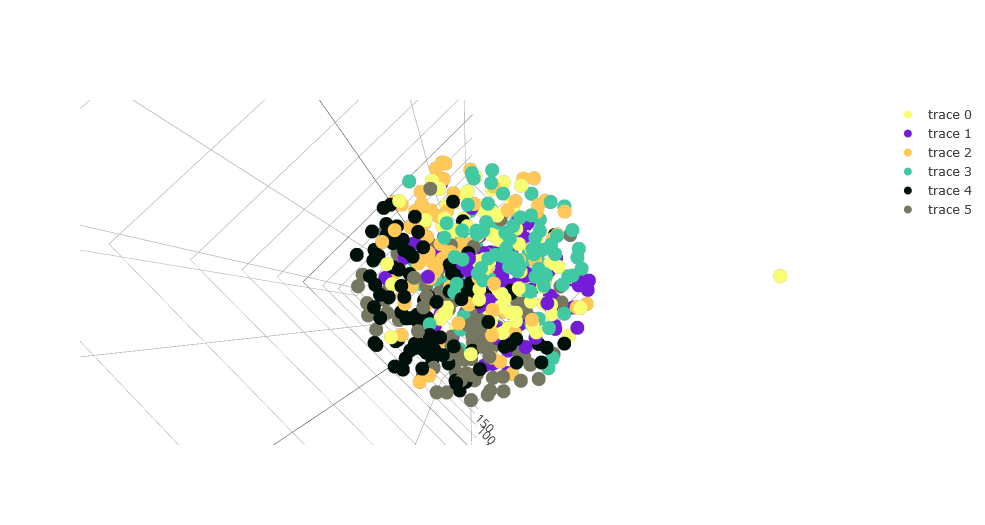
\includegraphics[width=.45\linewidth]{tsne-1-1} }}%
    \qquad
    \subfloat[Vista ravvicinata]{{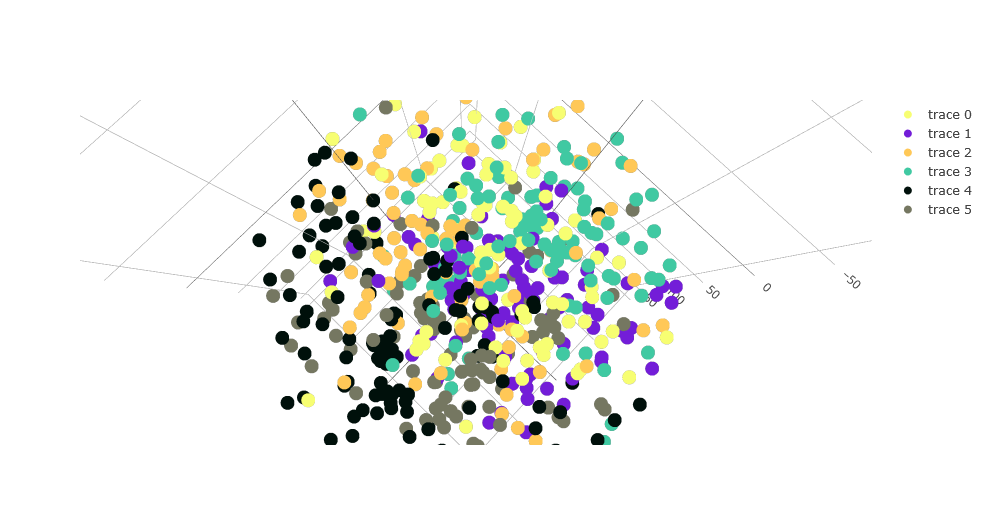
\includegraphics[width=.45\linewidth]{tsne-1-2} }}%
    \caption{Riduzione della term document matrix da forma (2400, 4640) a forma (2400, 3) via tSNE. }%
    \label{fig:tsne1}%
\end{figure}

Si vede in Figura 1 come articoli dello stesso tema sono abbastanza distaziati tra loro e sparsi nell'agglomerato di
articoli.\par

\qquad
\qquad




Successivamente si \'e riprovato attraverso la stessa pipeline con in pi\'u la Latent Dirichlet (LDA), impostando come parametri n\_components \footnote{numero di topic latenti che LDA dovrebbe individuare} a 6 e learning\_decay\footnote{parametro usato per regolare il ''learning rat\'e', che si consiglia imposare nel range (0.5, 1] per garantire la convergenza asintotica.} al valore di default.



%quelli della classe CountVectorizer: ngram\_range\footnote{ampiezza intervallo degli n-grammi da considerare}, min\_df\footnote{minimo document frequency, cio\'e il minimo numero di volte che una parola deve apparire in un documento affinch\'e questa venga inclusa nel vettore di conteggio.}, max\_df\footnote{controparte di min\_df}; e quelli del classificatore via Alberi: min\_samples\_leaf\footnote{indica il numero di osservazioni minimo per ogni foglia}, max\_depth\footnote{indica la profondit\'a massima dell'albero}.




\begin{figure}%
    \centering
    \subfloat[Vista normale]{{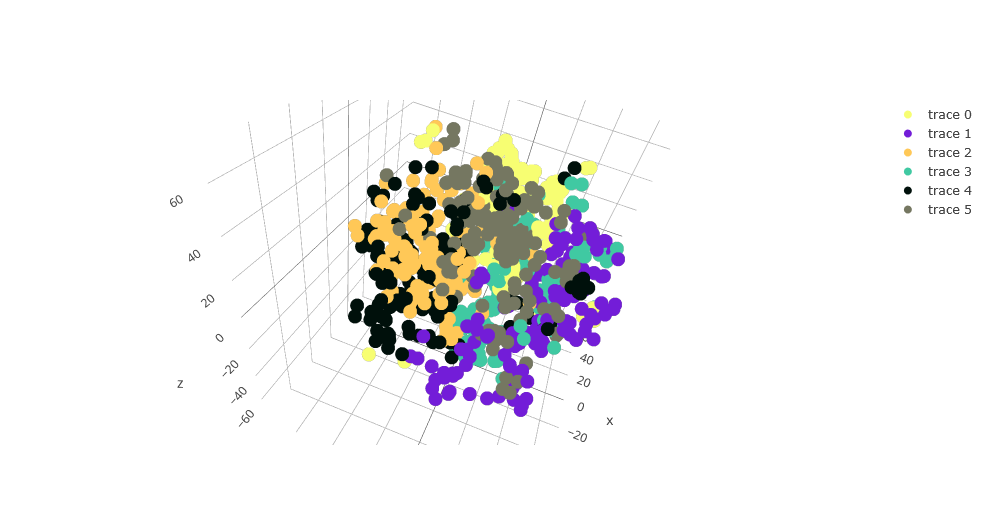
\includegraphics[width=.45\linewidth]{tsne_ottimizzato-1} }}%
    \qquad
    \subfloat[Vista ravvicinata]{{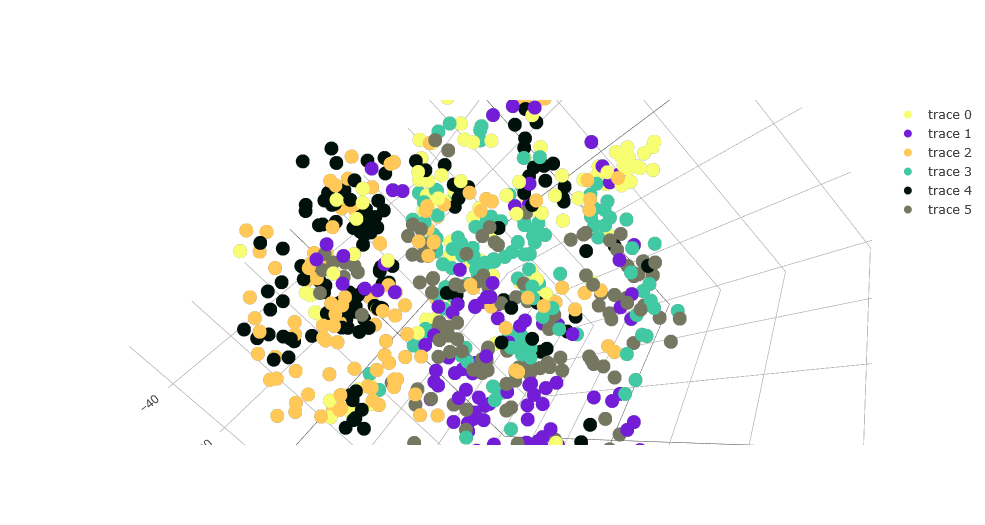
\includegraphics[width=.45\linewidth]{tsne_ottimizzato} }}%
    \caption{Riduzione della matrice da forma (2400, 4640) a forma (2400, 3). }%
    \label{fig:tsne2}%
\end{figure}


A differenza della Figura 1 in questa figura (esplorazione interattiva
\footnote{https://plot.ly/create/?fid=cristi.gutzu:5\&fid=cristi.gutzu:6}) si vede come i diversi temi sono raggruppati in piccoli cluster sparsi in maniera pi\'u o meno uniforme lungo i tre assi, inoltre articoli dello stesso tema nella Figura 2 sembrano essere meno distanti tra loro. Sempre dalla Figura 2 si evince come un albero potrebbe essere una soluzione accettabile per il problema di classificazione.

\subsection{Prove}

Si \'e deciso di usare 3 configurazioni attraverso le quali efettuare le analisi, se ne possono vedere alcune caratteristiche nella Tabella 1.
%Si \'e deciso di mettere a confronto 3 configurazioni attraverso le quali si vede come l'accuratezza delle predizioni
%varia al variare della dimensione del training set. Nella seguente tabella si evincono le 3 configurazioni.

\def\checkmark{\tikz\fill[scale=0.3](0,.3) -- (.25,0) -- (1,.7) -- (.25,.15) -- cycle;}
\begin{table}[]
\centering
\begin{tabular}{llll}
\hline
\textbf{Pipeline} \textbackslash \textbf{Trasformation} & LDA-12 & LDA-48 & Term Frequency \\ \hline
T.D Matrix                  &    \checkmark    & \checkmark      & \checkmark    \\
LDA                       & \checkmark      & \checkmark      & x   \\
Classifier                & \checkmark      & \checkmark      & \checkmark     \\ \hline
\end{tabular}
\begin{tablenotes}
      \small
      \item
    \end{tablenotes}
\caption{  Configurazioni LDA-12 e LDA-48, indicano i modelli fittati con 12 e 48 componenti.}
\end{table}

Prima di iniziare le prove sono stati ottimizzati, per ogni configurazione, alcuni parametri dell'albero di decisione (profondit\'a massima e numero minimo di osservazioni per foglia.) effettuando una ricerca a griglia e massimizzando l'accuratezza sull'inisieme di validazione.
La prima prova effettuata riguarda la misurazione dell'accuratezza nel classificare al variare della dimensione dell'inisieme di training.
\vskip 0.2in
Dalla figura 3, si nota che tutte e tre le configurazioni hanno un andamento piuttosto simile se non quando l'insieme di training \'e abbastanza ristretto, come si vede a livello 15\% in questi casi le configurazioni con pi\'u features sembrano funzionare meglio.


\begin{figure}%
    \centering
    \subfloat{{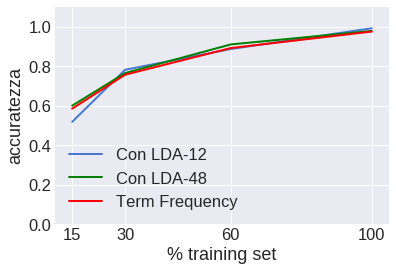
\includegraphics[width=.5\linewidth]{accuracy} }}%
    \caption{Performace modelli di classificazione sul test set in funzione della dimensione del training set.}%
\end{figure}

Successivamente sono state misurate le performance delle 3 configurazioni usando l'intero insieme di training, sia dal punto di vista dell'accuratezza\footnote{calcolata sull'insieme di test} che dal punto di vista dei tempi di esecuzione. I risultati sono riassunti nelle tabelle 2 e 3.

\begin{table}[]
    \centering
\begin{tabular}{ll}
\hline
Rappresentazione & Accuratezza      \\ \hline
Dummy            & 17.8 \%          \\
LDA-12           & \textbf{99.2 \%} \\
LDA-48           & 97.8 \%          \\
Term Frequency   & 98.5 \% \\ \hline
\end{tabular}
    \caption{Risultati utilizzando i diversi modelli di rappresentazione con l'intero training set.}%
\end{table}

\begin{table}[]
    \centering
\begin{tabular}{lll}
\hline
Rappresentazione & Tempi trasf. & Tempi class. \\ \hline
LDA-12           & 99.55 s & \textbf{0.02 s} \\
LDA-48           & 141.54 s & 0.07 s   \\
Term Frequency   & \textbf{5.29 s} & 1.93 s \\ \hline
\end{tabular}
    \caption{Tempi misurati sulla trasformazione delle variabili e sulla classificazione.}%
\end{table}


Come si nota in Tabella 2, tutte le rappresentazioni superano abbondantemente la soglia definita dalla baseline, in particolare, la LDA-12 risulta performare meglio dal punto di vista dell'accuratezza classificando gli articoli dell'insieme di test.

\vskip 1.2in

Siccome l'accuratezza, che misura la qualit\'a complessiva del modello, risulta molto buona, ci si \'e chiesti se il classificatore, con la configurazione migliore, si comporta altrettanto bene anche per le singole classi, per verificarlo abbiamo calcolato ulteriori misure, riportate in Tabella 4.


%
%    'lda__n_components': 12,
%    'lda__learning_decay': 0.7,
%    'count_mx__ngram_rang\'e: (1, 3),
%    'count_mx__min_df': 10,
%    'count_mx__max_df': 0.5,
%    'classifier__min_samples_leaf': 1,
%    'classifier__max_depth': 22




\begin{table}[]
\centering
\begin{tabular}{lllll}
\hline
Categoria    & precision & recall & f1   & support \\ \hline
Cronaca      & 1.00   &   1.00    &  1.00  & 107      \\
Cultura      & 0.98      & 0.98   & 0.98 & 88      \\
Economia     & 1.00      & 0.98   & 0.99 & 99      \\
Politica     & 1.00      & 0.98   & 0.99 & 107      \\
Sport        & 0.98      & 1.00   & 0.99 & 96      \\
Tech         & 0.99      & 1.00   & 1.00 & 103      \\ \hline
micro avg    & 0.99      & 0.99   & 0.99 & 600     \\ \hline
macro avg    & 0.99      & 0.99   & 0.99 & 600     \\ \hline
weighted avg & 0.99      & 0.99   & 0.99 & 600    \\  \hline
\end{tabular}
    \caption{Report metriche sul classificatore stimato con LDA-12.}%

\end{table}



Si osserva dalla tabella che le metriche: precisione, richiamo, f1; sono molto alte per tutte le classi e quindi in accordo con l'accuratezza confermano la validit\'a del modello utilizzato.


\section{Conclusioni}

Dai risultati delle analisi si vede che il modello basato sulla rappresentazione con LDA \'e comparabile al modello basato sulla rappresentazione con Term Frequency dal punto di vista dell'accuratezza, inoltre se confrontiamo i tempi di esecuzione, presenti nella Tabella 3, notiamo che il guadagno otteuto riducendo la dimensione delle features \'e annullato dal tempo che \'e necessario per trasformare i dati; ci\'o \'e valido perlomeno nell'ambiente python con le funzioni e classi della libreria scikitlearn che sono state utilizzate, concludiamo dicendo che riteniamo sarebbero opportune ulteriori analisi utilizzando pacchetti che ottimizzino il processo di stima del modello LDA.

Nota: il dataset \'e composto soprattutto da articoli caricati intorno ai mesi di maggio e giugno 2019 e perciò, vista la variabilit\'a dei termini, dovuta al tempo, il modello adattato con questo insieme di training potrebbe non dare risultati altrettanto buoni se utilizzato per classificare articoli troppo distanti nel tempo.

% il modello con LDA riduce lo spazio delle variabili riducendo i costi computazionali nel processo di classificazione, che per\'o vengono aumentati

%
%I parametri citati sopra, sono stati ottimizzati utilizzando la tecnica del Random Search attraverso la funzione di precisione relativa al classificatore:
%
%$\psi\colon \mathbf{g}(TP,FP) \rightarrow [0,1]$ con $ \mathbf{g}(TP,FP) = TP / (FP + TP)$.
%
%Inizialmente si \`e pensato che utilizzare le stopword generali della lingua inglese fosse sufficiente per eliminare le
%parole che non portano informazione, e di conseguenza aumentare il parametro di interesse M.A.P; i risultati
%non sono stati molto soddisfacenti, abbiamo quindi optato per l'utilizzo di stopword cliniche, cio\`e stopword utilizzate
%soltato in ambito clinico/medico \cite{stopword_cliniche}.

\begin{thebibliography}{9}

\bibitem{LDA}
David m. Blei, Andrew Y, Ng, and Michael I. Jordan, 2013, Latent Dirichlet Allocation

\bibitem{tree}
Hastie T., 2016, Introduction to Statistical Learning, Decision Trees

\bibitem{NGRAM}
Ceron, Curini, Iacus, 2014,  Social Media e Sentiment Analysis.


\end{thebibliography}


\end{document}
